The dating is done by computing the distance between a small set of articles and each year. The prediction is the year for which the distance is the smallest.

\begin{figure}[H]
    \begin{minipage}[b]{0.3\linewidth}
        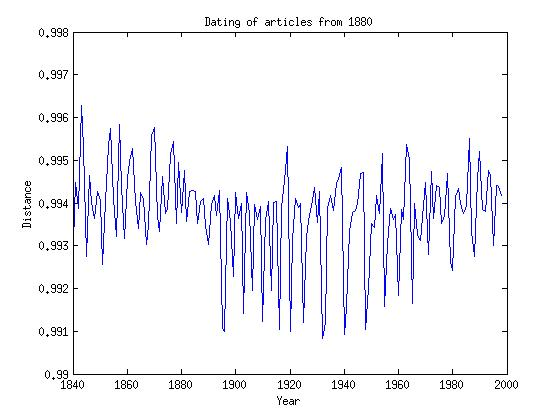
\includegraphics[scale=0.25]{Pictures/date_articles/distance1/dating1880.jpg}
        \caption{Dating articles from 1880 with the basic distance}
    \end{minipage}\hfill
    \begin{minipage}[b]{0.3\linewidth}
        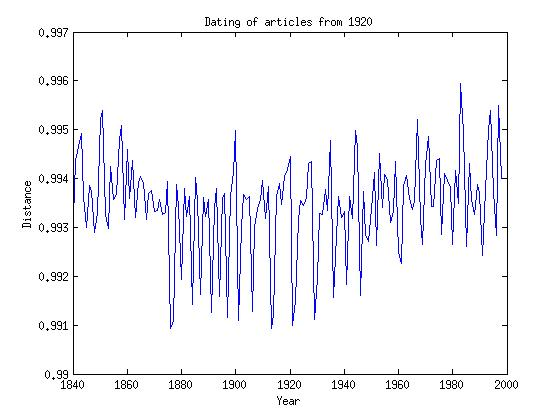
\includegraphics[scale=0.25]{Pictures/date_articles/distance1/dating1920.jpg}
        \caption{Dating articles from 1920 with the basic distance}
    \end{minipage}\hfill
    \begin{minipage}[b]{0.3\linewidth}
	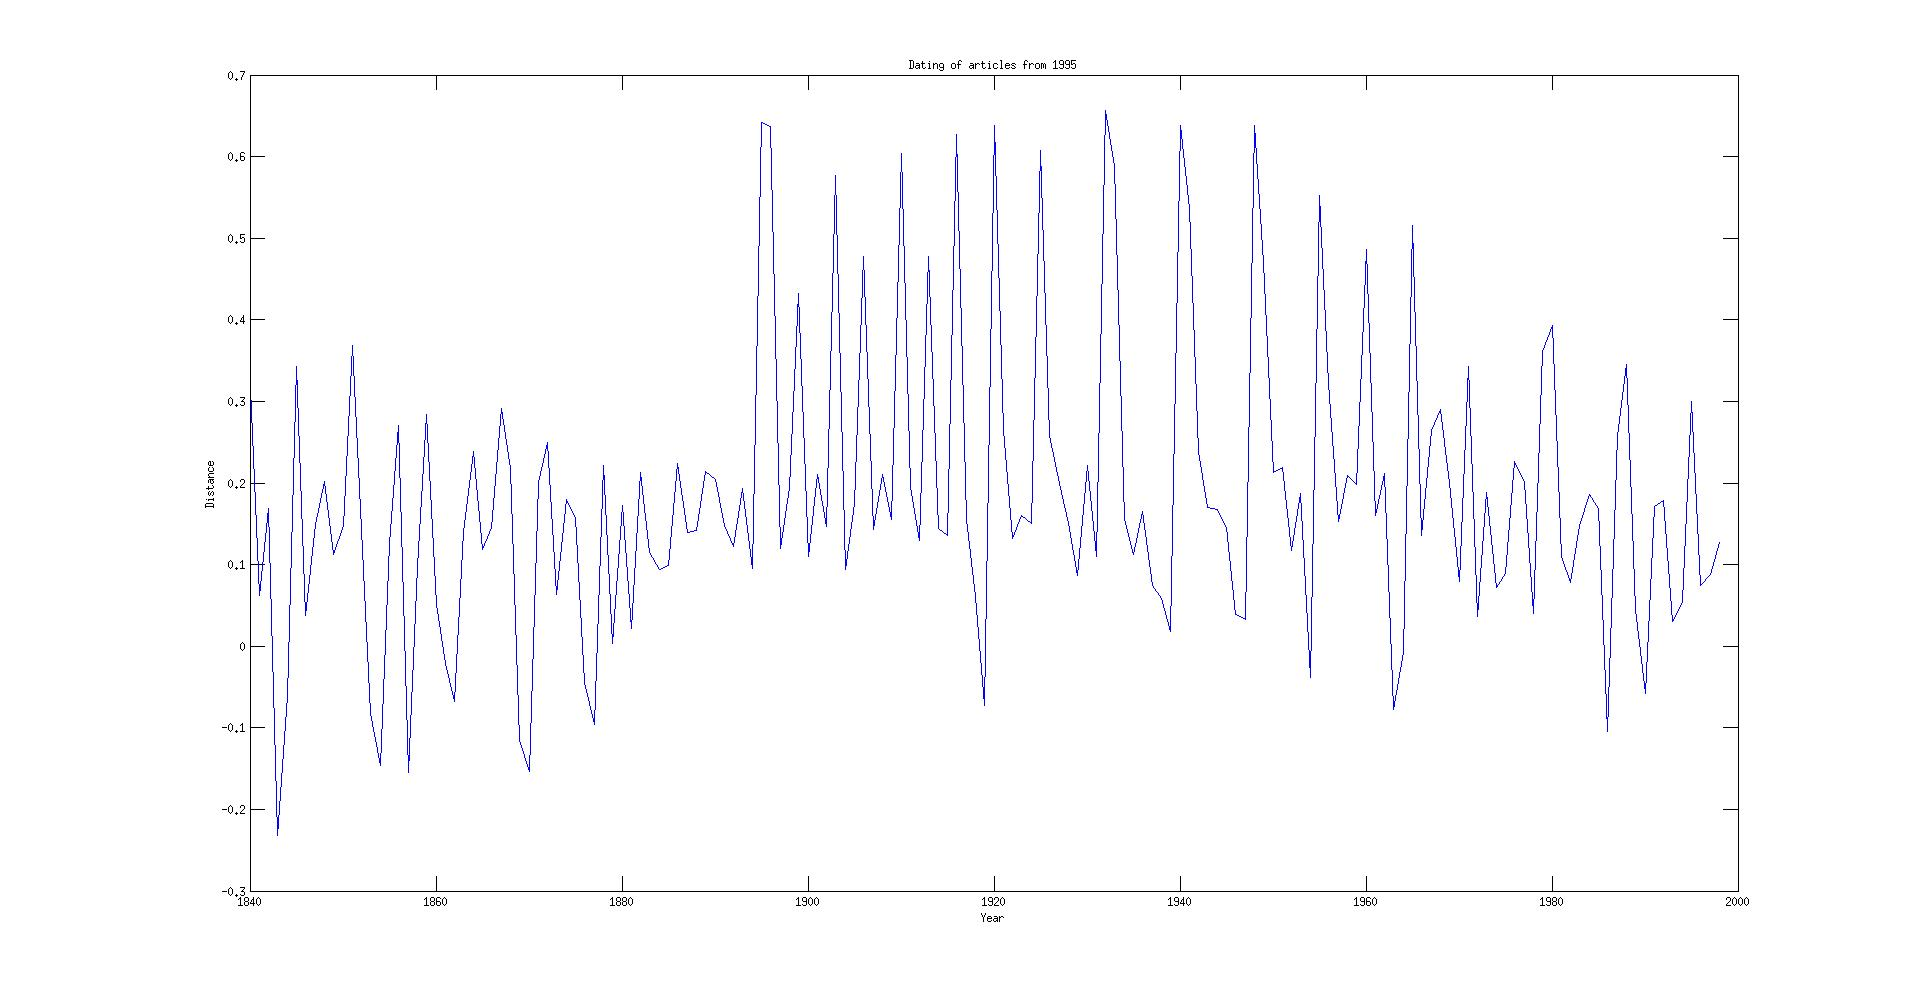
\includegraphics[scale=0.25]{Pictures/date_articles/distance1/dating1995_corrected.jpg}
        \caption{Dating articles from 1995 with the basic distance}
    \end{minipage}
    \label{date_d1}
\end{figure}
With the basic metric, the distances look very random. The prediction given by the example on figure \ref{date_d1} is 1843 for articles from 1995.

In our opinion, this "sawteeth" behavior can be explained because the amount of words suddenly drop in certain years. Indeed, the basic distance is subject to the number of words in each year and knowing that in 1840's years there are less words in the others and that between 1917 and 1919 and in 1998 there are less articles too, the predicted year will almost always one of the previous ones.
